\chapter{Background}
\label{chap:bg}

This chapter gives the background of \betrfs.
\betrfs is a file system based on write-optimized \bets, which offers good
random write performance by cascading writes in batches.
Alsp, \betrfs adopts full-path indexing or relative-path indexing for spatial
locality.
This chapter first introduces \bets and then the full-path-indexed or
relative-path-indexed schema of \betrfs.

\section{\bets}
\label{sec:bet}

\bets~\citep{bet,betlogin} are \btrees, augmented with buffers in non-leaf
nodes.
New writes are injected as messages into the buffer of the root node of a \bet.
When a node's buffer becomes full, messages are flushed from that node's buffer
to one of its children's buffers.
The leaves of the \bet store key/value pairs, as in a \btree.
Besides checking key/value pairs in the leaves, point and range queries in a
\bet must check related messages in the buffers along the root-to-leaf path.

\begin{table}[t]
    \centering
    \begin{tabular}{c | c c c}
        \hline
        Data Structure & Insert & Point Query & Range Query \\
        \hline
        \hline
        \btree & $O(log_{B}{N})$ & $O(log_{B}{N})$ & $O(log_{B}{N} + k/B)$\\
        \hline
        \bet & $O({log_{B}{N}}/{\varepsilon B^{1 - \varepsilon}})$ & $O({log_{B}{N}}/{\varepsilon})$ & $O({log_{B}{N}}/{\varepsilon} + k/B)$ \\
        \hline
        \bet ($\varepsilon=0.5$) & $O(log_{B}{N}/{\sqrt{B}})$ & $O(log_{B}{N})$ & $O(log_{B}{N} + k/B)$ \\
        \hline
    \end{tabular}
    \caption[The asymptotic IO costs of \btrees and \bets]{\label{tab:betbtree}
        The asymptotic IO costs of \btrees and \bets.}
\end{table}

\bets are asymptotically faster than \btrees, as shown in
Table~\ref{tab:betbtree}.
Consider a \btree with $N$ key/value pairs and each node can hold $B$ keys.
The tree has fanout $B$, so its height is $O(log_{B}{N})$.
Inserts and point queries need to fetch all nodes along the root-to-leaf path,
resulting in $O(log_{B}{N})$ IOs.
A range query for $k$ key/value pairs requires $O(log_{B}{N} + k/B)$ IOs.

For comparison, a \bet with node size $B$ has fanout $B^{\varepsilon}$, where
$0 < \varepsilon \leq 1$.
Therefore, pivot keys in a non-leaf node consume $B^{\varepsilon}$ space and
the remaining $(B - B^{\varepsilon})$ space is used for buffers.
The \bet has height $O(log_{B}{N}/\varepsilon)$, because the fanout is
$B^{\varepsilon}$.
A point query fetches all nodes along the root-to-leaf path with
$O(log_{B}{N}/\varepsilon)$ IOs and a range query for $k$ key/value pairs
requires $O({log_{B}{N}}/{\varepsilon} + k/B)$ IOs.
On the other hand, the cost of an insert consists of injecting the message into
the root node and flushing the message down at each level.
When flushing, \bets has $O(B - B^{\varepsilon})$ messages and $B^{\varepsilon}$
children.
Thus, at leave one child can receive at least
$O((B - B^{\varepsilon})/B^{\varepsilon}) = O(B^{1 - \varepsilon})$ messages.
Therefore, the amortized cost of an insert in one flush is
$O(1/B^{1 - \varepsilon})$.
As an insert must be flushed $O(log_{B}{N}/\varepsilon)$ times, the amortized
cost of an insert is $O({log_{B}{N}}/{\varepsilon B^{1 - \varepsilon}})$.
A \bet with $\varepsilon = 1$ is equivalent to a \btree.
And if we pick $\varepsilon = 1/2$, the point and range query costs of the \bet
become $O(log_{B}{N})$ and $O(log_{B}{N} + k/B)$, which is the same as a \btree,
but the insert cost becomes $O(log_{B}{N}/{\sqrt{B}})$, which is faster by a
factor of $\sqrt{B}$.

One important change in \bets is that the IO costs for point queries and inserts
are asymmetric.
In \btrees, if an application want to update the old value associated with a
key, it must perform a point query to get the old value before inserting.
However, in \bets, this read-before-write behavior degrades update
performance to point query performacne.

\bets support ``upserts'' to avoid read-before-write.
An upsert injects a message with the key and a delta into the buffer of the root
node.
When the upsert message is flushed to the leaf, it updates the value associated
with the key with a user-specified function and the delta in the message.
With upsert messages, queries need to compute value on the fly, however, this
doesn't change the IO costs of queries.
On the other hand, updating an old value becomes as fast as an insert.

\section{\betrfs with full-path indexing}
\label{sec:fpi}

\begin{figure}
    \centering
    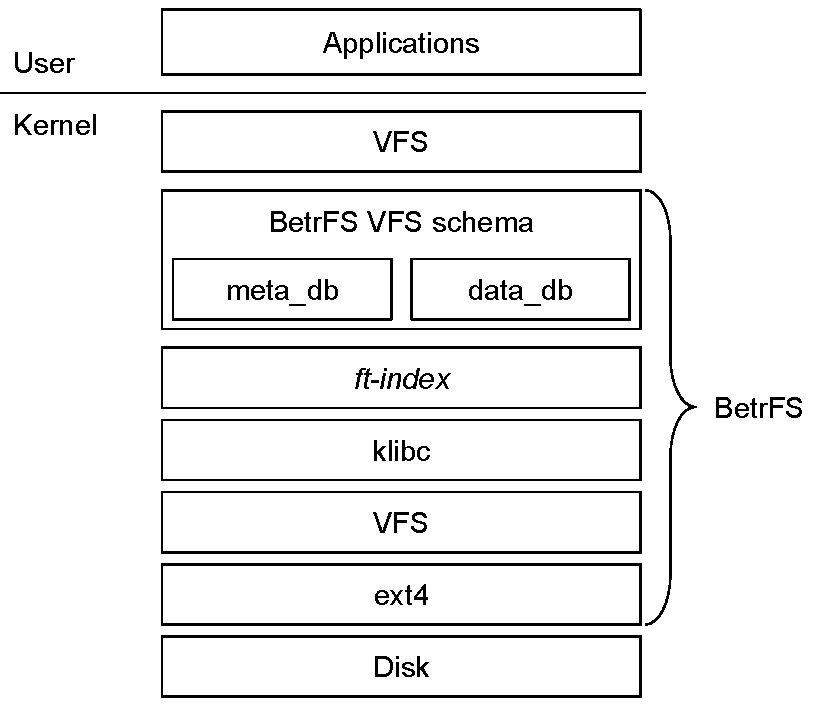
\includegraphics{proposal/fig/betrfs}
    \caption[The \betrfs architecture]{\label{fig:betrfs}
        The \betrfs architecture.}
\end{figure}

\betrfs~\citep{betrfs1,betrfs1tos} is a Linux in-kernel file
system built upon \fti~\citep{fti}, a key/value store that implements \bets and
exposes a key/value interface similar to BerkelyDB.
The architecture of \betrfs is shown in Figure~\ref{fig:betrfs}.
\betrfs interacts with \fti through point operations, such as \texttt{put},
\texttt{get} and \texttt{del}, as well as range queries with cursors
(\texttt{c\_get} with DB\_SET\_RANGE and DB\_NEXT).
\betrfs also uses the transaction interface of \fti to execute multiple
operations atomically.
A redo log and periodic checkpoints (every 60 seconds) in \fti ensure that
changes can be made persistent on the underlying storage media.

\Fti cannot be integrated into a Linux kernel module easily because
it is a userspace library that assumes libc functions and system calls.
We built a shim layer called \texttt{klibc} which implements all functions \fti
requires.
By implementing those functions in \texttt{klibc} instead of directly modifying
\fti, we are able to migrate \fti into the kernel module intact.

\betrfs uses two key/value indexes to store the metadata and data in the file
system.
One \texttt{meta\_db} maps full-paths to \texttt{struct stat} structures.
Another \texttt{data\_db} maps (full-path plus block number) to 4KB blocks.
When the VFS (Virtual File System) needs metadata, \betrfs queries
the \texttt{meta\_db} with the full-path and constructs the corresponding inode
from the \texttt{struct stat}.
Likewise, when a dirty inode needs to be written, the \texttt{struct stat} is
assembled from the inode and written to the \texttt{meta\_db} with the
full-path key.
Blocks of a file are fetched and written by the full-path and the indexes of
blocks.
Although other block granularity is possible, 4KB is the natural block size
because it is the same as the page size in the Linux page cache.

Full-path indexing ensures locality even with file system aging~\citep{betrfs3}.
After \betrfs fetches one block of a file from the disk, all nodes along the
root-to-leaf path are present in memory.
And with full-path indexing, all keys under one directory are contiguous in the
keyspace, which means a subsequent fetch of some other block in the same file or
another file under than same directory is likely to be resolved in memory,
which significantly increases performance and IO efficiency.

\betrfs can write to a block without fetching the old block to memory, avoiding
expensive read-before-write described in Section~\ref{sec:bet}.
Conventional file systems must read the old block from the disk to the page
cache before writing to that block (a complete overwrite can be done without
fetching the old block, but it is not implemented in any file system).
However, \bets have asymmetric read and write costs, so read-before-write should
be avoided.
In \betrfs, if the corresponding block is not in memory, an upsert message,
which describes the offset, length and content of this write, is injected into
the \bet.
When this message is flushed to the leaf, the change is applied to the old
block.

The full-path-index \betrfs (\betrfsOne) has great random write performance
and locality.
Recursive greps run 3.8x faster than in the best standard file system.
File creation runs 2.6x faster.
Small, random writes to a file run 68.2x faster.

However, range operations have predictably miserable performance.
Deleting a Linux source directory takes 46 seconds and renaming it takes
21 seconds in \betrfsOne, both because the file system has to perform one
operation for each key.
We solved the deleting problem with a range-delete message that nullifies all
messages within a range, but the renaming remains a diffcult problem.

\section{\betrfs with relative-path indexing}
\label{sec:rpi}

\begin{figure}
    \begin{subfigure}{.5\textwidth}
        \centering
        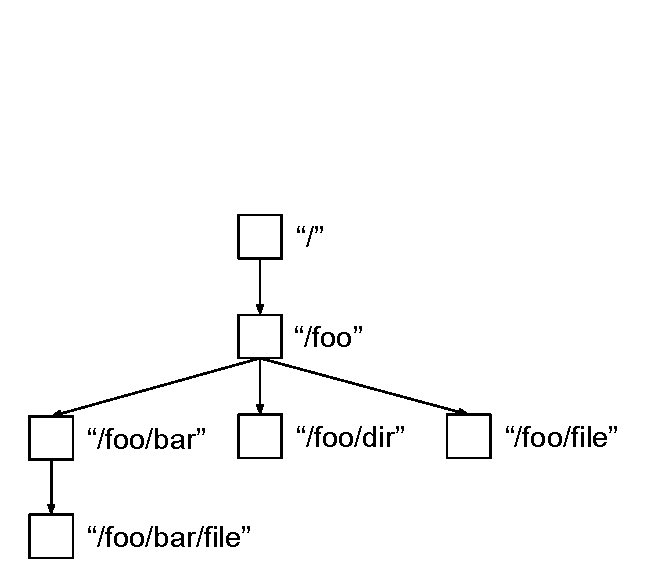
\includegraphics[width=.9\linewidth]{proposal/fig/FPI}
        \caption{\label{subfig:FPI} Full-path indexing.}
    \end{subfigure}
    \begin{subfigure}{.5\textwidth}
        \centering
        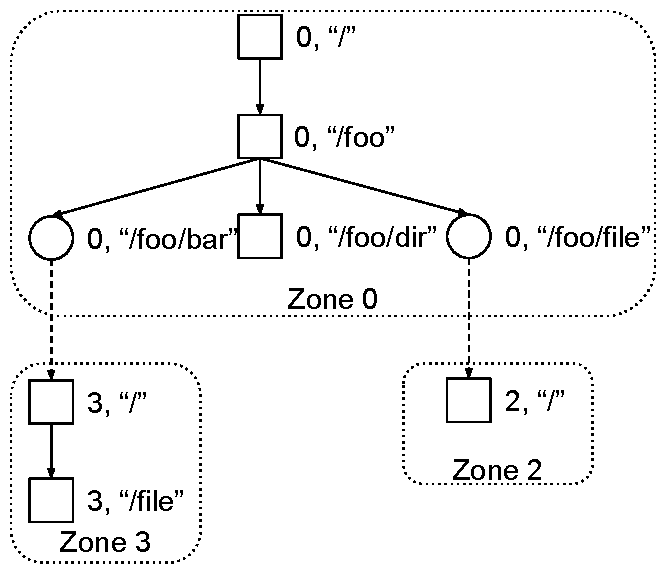
\includegraphics[width=.9\linewidth]{proposal/fig/RPI}
        \caption{\label{subfig:RPI} Relative-path indexing.}
    \end{subfigure}
    \caption[Full-path indexing and relative-path indexing]{\label{fig:FPIRPI}
        Full-path indexing and relative-path indexing.}
\end{figure}

\betrfsTwo~\citep{betrfs2,betrfs2tos} backed away from full-path indexing and
introduced relative-path indexing, which is also called zoning.
Relative-path indexing partitions the directory hierarchy into zones.
Each zone has a zone ID (analogous to an inode number and the root zone is
always 0) and a single root file or directory.
All file or directory in a zone is indexed relative to the zone root.
If the file or directory is the root of another zone, the entry contains that
zone ID to redirect queries.

Figure~\ref{fig:FPIRPI} shows the same directory hierarchy under full-path
indexing and relative-path indexing.
In Figure~\ref{subfig:RPI}, when querying the key/value store for file
``/foo/file'' with key (0, ``/foo/file''), the file system gets a special value
indicating it is the root of Zone 2.
Subsequently, the file system queries the key/value store with key (2, ``/'')
and gets the right value.
Similary, the file system notice the key for directory ``/foo/bar'' is
(3, ``/'').
Therefore, when querying for file ``/foo/bar/file'', it uses key (3, ``/file'').

\begin{figure}[t]
    \centering
    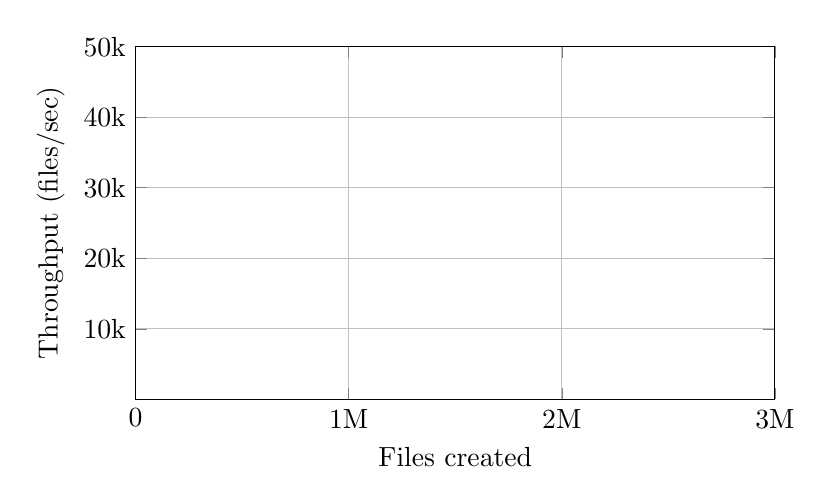
\begin{tikzpicture}
        \begin{axis}[
            xlabel={Files created},
            ylabel={Throughput (files/sec)},
            xmin=0,
            xmax=3000000,
            ymin=10,
            ymax=50000,
            mark repeat=10,
            xtick={0,1000000,2000000,3000000},
            xticklabels={0,1M,2M,3M},
            ytick={10000,20000,30000,40000,50000},
            yticklabels={10k,20k,30k,40k,50k},
            grid=major,
            scaled x ticks=false,
            scaled y ticks=false,
            legend cell align=left,
            transpose legend,
            height=.5\linewidth,
            width=.8\linewidth,
        ]
        \addTokubenchPlot{betrfs3};
        \end{axis}
    \end{tikzpicture}
    \caption[Zone maintainance cost in TokuBench]{Cumulative file creation
        throughput during the Tokubench benchmark (higher is better).
        \betrfsThree has a sudden performance drop because of zone splitting.}
    \label{fig:tokuzone}
\end{figure}

Relative-path indexing tries to balance locality and rename performance through
a target zone size.
Larger zones mean better locality because full-path indexing is still maintained
within the zone, while smaller zones impose a lower bound on renaming latency
because no rename needs to mutate more key/value pairs than a zone.

Relative-path indexing made renames on \betrfsTwo almost as fast as inode-based
file system and recursive-directory trawversals almost as fast as \betrfsOne.

However, relative-path indexing also imposes zone maintainance costs on other
file system operations.
For instance, in Figure~\ref{fig:tokuzone}, two-thirds of the way through the
TokuBench benchmark, \betrfsThree (\betrfsThree is \betrfsTwo with some bug
fixes) shows a sudden, precipitous drop in cumulative
throughput for small file creation, because the file system performs a huge
amount of zone splitting.

Furthermore, relative-path indexing also has bad worst-case performance.
It is possible to construct arrangements of nested directories that will each
reside in their own zone.
Reading a file in the deepest directory will require reading one zone per
directory (each withits own I/O).
Such a pathological worst case is not possible with full-path indexing in a
\bet, and an important design goal for \betrfs is keeping a reasonable bound on
the worst cases.

Finally, zones break the clean mapping of directory subtrees onto contiguous
ranges of the key space, preventing us from using range-messages to implement
bulk operations on entire subtrees of the directory hierarchy.

